In \textsc{pedersen hash}, we have depicted the circuit used to compute (equatio \ref{eq-ped}). Each \textsc{multiplication} box returns one term of the sum. 
%that takes, per bit, that many constraints (of a circuit). 

\begin{figure}[h]
	\centering
	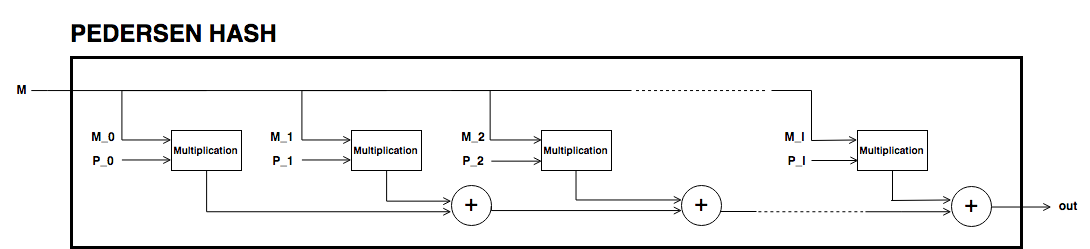
\includegraphics[scale=0.4]{Diag/Ped_Hash.png}
	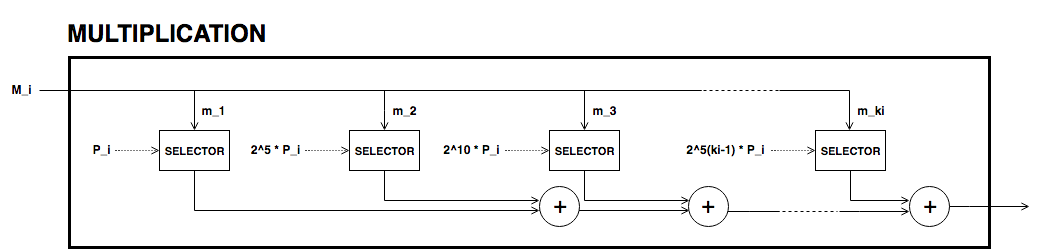
\includegraphics[scale=0.4]{Diag/Ped_Hash_Multiplication.png}
\end{figure}

As the set of generators are fixed, we can precompute its multiples and use 4-bit lookup windows to select the right points. This is done as shown in next circuit \textsc{selector}.

\begin{figure}[h]
	\centering
	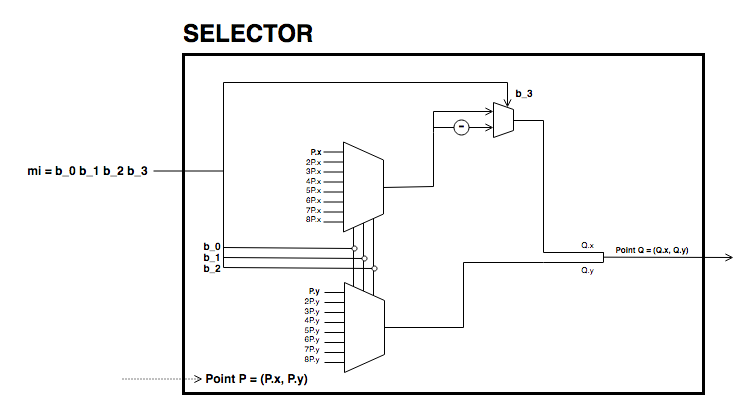
\includegraphics[scale=0.5]{Diag/Ped_Hash_Multiplication_selector.png}
\end{figure}

The circuit receives as input a 4-bit chunk. The first three bits are used to select the right multiple of the point and last bit decides the sign of the point. Recall that negation on a point of a twisted Edwards curve corresponds to negation of its first coordinate. 